\section{化学性质}

\subsection{亲核取代}

衍生物的亲核取代反应机理上为先加成、再消去。


\begin{center}
    \small
    \schemestart
    \chemfig{R-[:30]C(=[:90]O)-[:-30]L} \arrow{->[\ch{Nu\mch}]} \chemfig{R-C(-[:90]\ch{O\mch})(-[:-90]\ch{Nu})-L} \arrow{->[-L]} \chemfig{R-[:30]C(=[:90]O)-[:-30]Nu}
    \schemestop
\end{center}

\subsubsection{酰卤的水解}

水解反应的机理为亲核取代,不同衍生物的反应活性是:

\begin{equation*}
    \mbox{酰卤} > \mbox{酸酐} > \mbox{酯} > \mbox{酰胺}
\end{equation*}

酸酐的水解需要酸催化,酯还需要加热,酰胺还需要回流。酸催化的作用时增加碳上的正电荷。使得反应物更容易被水中的\ch{OH\mch}进攻。

\begin{center}
    \scriptsize
    \schemestart
    \chemfig{R-[:30]C(=[:90]O)-[:-30]L} \arrow{->[\ch{H\pch}]} \chemfig{R-[:30]C(=[:90]OH\ch{\pch})-[:-30]L} \arrow{->[\ch{OH\mch}]} \chemfig{R-C(-[:90]OH\ch{\pch})(-[:-90]OH\ch{\mch})-L} 
    \arrow{->[\ch{-HL}][-\ch{H\pch}]} \chemfig{R-[:30]C(=[:90]O)-[:-30]OH}
    \schemestop
\end{center}


\subsubsection{酰卤制备酚酯}

酚酯一般难以用酸和酚直接制备,需要使用酰卤。

\begin{center}
    \scriptsize
    \schemestart
    \chemfig{R-[:30]C(=[:90]O)-[:-30]Cl} \+ \chemfig{*6(-=-(-OH)=-=)} \arrow{->}
    \schemestop
\end{center}


\subsubsection{氨解反应和氨基的保护}

\begin{center}
    \scriptsize
    \schemestart
    \chemfig{*6(-=-=(-NH_2)-=)} \arrow{->[\chemfig{CH_3-C(=[:90]O)-Cl}][或酸酐]}[,2.3] \chemfig{*6(-=-=(-NH-[:0]C(=O)-[:0]CH_3)-=)}
    \schemestop
\end{center}

\subsubsection{与\ch{RMgX}的反应}

\begin{center}
    \scriptsize
    \schemestart
    \chemfig{R-[:30]C(=[:90]O)-[:-30]Cl} \arrow{->[\ch{RMgCl}]}[,1.2] \chemfig{R-C(-[:90]OMgCl)(-[:-90]R)-Cl} \arrow{->[-\ch{MgCl2}]}[,1.4] \chemfig{R-[:30]C(=[:90]O)-[:-30]R}
    \schemestop
\end{center}

生成的酮可以进一步和格氏试剂反应,但是第一步反应的活性更强,因此可以通过控制格氏试剂的量来控制反应的数量级。

如果是酯与格氏试剂反应,则更容易变为最终的醇。因为第一步酯和格氏试剂的反应本身比酰卤困难得多。如果想让酯停留在第一个取代的阶段,则需要控制空间位阻效应。

\subsection{还原反应}

另外,这些衍生物还可以发生还原反应。还原反应的活性依然是
\begin{center}
    酰卤>酸酐>酯>酰胺    
\end{center}

\begin{center}
    \small
    \schemestart
    \chemfig{R-[:30]C(=[:90]O)-[:-30]Cl}  \arrow{->[\ch{LiAlO4}]} RCHO \arrow{->} \ch{RCH2Cl}
    \schemestop
\end{center}

\begin{center}
    \small
    \schemestart
    \chemfig{R-[:30]C(=[:90]O)-[:-30]NH_2}  \arrow{->[\ch{LiAlO4}]} \ch{RCH2NH2}
    \schemestop
\end{center}

$\ce{NaNH4}$只还原酰卤。

\begin{center}
    \small
    \schemestart
    \chemfig{R-[:30]C(=[:90]O)-[:-30]NH_2} + $\ce{HCl}$ \arrow \chemfig{R-[:30]C(=[:90]O)-[:-30]\charge{90:3pt=+}{N}H_3}
    \schemestop
\end{center}

\subsection{Gahmel合成法}


\begin{center}
    \scriptsize
    \schemestart
    \chemfig{*6(-=*5(-C(=O)-NH-C(=O)-)-=-=)} \arrow{->[$\ce{KOH}$ ]}  \chemfig{*6(-=*5(-C(=O)-{N^-}-C(=O)-)-=-=)}  \arrow{->[$\ce{RCl}$ ]} \chemfig{*6(-=*5(-C(=O)-NR-C(=O)-)-=-=)} \arrow{->[$\ce{H2O}$ ]} \chemfig{*6(-=(-COOH)-(-COOH)=-=)} \+ $\ce{RNH2}$ 
    \schemestop
\end{center}

\subsection{脱水反应}

\begin{center}
    \small
    \schemestart
    \chemfig{R-[:30]C(=[:90]O)-[:-30]NH_2} \arrow{->[$\ce{B2O4}$ ]} \chemfig{R-C~N}
    \schemestop
\end{center}


\subsection{Hoffmam降级反应}

\begin{center}
    \small
    \schemestart
    \chemfig{R-[:30]C(=[:90]O)-[:-30]NH_2} \arrow{->[$\ce{Br2}$ ][$\ce{NaOH}$ ]} \chemfig{R-[:-30]N=[:30]C=[:30]O} \arrow{->[$\ce{H2O}$ ][-$\ce{CO2}$ ]} \chemfig{R-NH_2}
    \schemestop
\end{center}


邻氨基苯甲酸在工业上就是通过这个反应制备的。 

\begin{figure}[H]
    \centering
    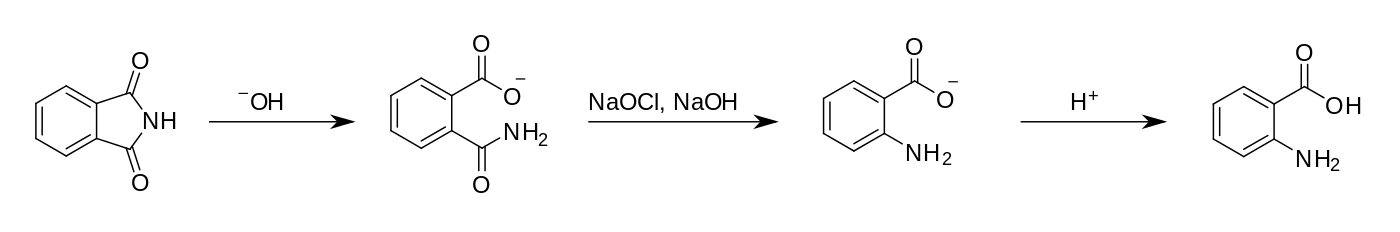
\includegraphics[width=1.0\textwidth]{img/1400px-Anthranilic_acid_synthesis_01.svg.png}
\end{figure}